\documentclass[a4paper]{article}

\title{Rapport de stage}
\usepackage[utf8]{inputenc}
\usepackage[francais]{babel}
\usepackage{amsmath}
\usepackage{eufrak}
\usepackage{graphicx}
\usepackage{listings}

\newtheorem{Rem}{Remarque}[subsection]
\newtheorem{Ex}{Exemple}[subsection]
\newtheorem{Def}{Définition}
\newtheorem{Prop}{Proposition}
\newtheorem{Th}{Théorème}

\begin{document}
\author{Quentin Honoré}
\date{}
\maketitle
\newpage
\tableofcontents
\newpage

\section{Les plans projectifs finis}
\subsection{Définition}
Soit P l'ensemble fini des points et D $ \subseteq \mathfrak{P} $ l'ensemble des droites.
(P,D) est un plan projectif fini si et seulement si: \\
$\cdot$ Par deux points distincts passe une unique droite. \\
$\cdot$ Deux droites distinctes se coupent en un unique point. \\
$\cdot$ Il existe un quadrilatère (4 points tels que pour chaque triplet, les 3 points ne sont pas alignés).

\begin{Rem}
$\cdot$ Les 2 premières propositions sont symétriques. \\ 
\end{Rem}
  
\begin{Ex}
  On va construire un plan projectif fini d'ordre 3 (3 points par droite, et 3 droites se coupent en chaque point). On construit d'abord un quadrilatère. Puis on construit les intersections entre les 2 droites horizontales, les 2 droites verticales et les diagonales. Ces intersections sont les intersections "à l'infini".
\begin{center}
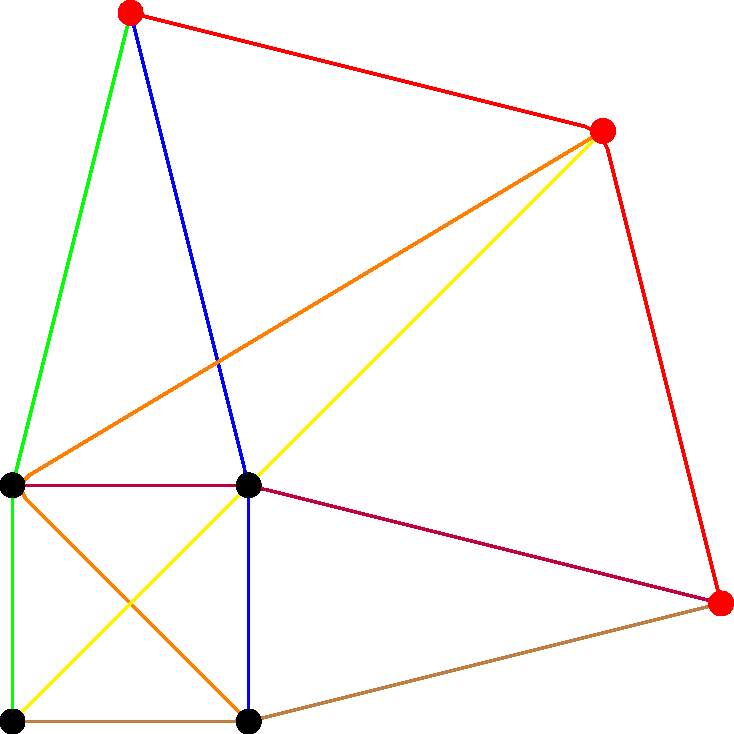
\includegraphics{test_tikz.pdf}
\end{center}
Les 3 propositions sont bien vérifiées.
\end{Ex}

\begin{Ex}
Le jeu du Dobble est un bon exemple de plan projectif fini. Si vous ne le connaissez pas, le Dobble est un jeu composé de 57 cartes sur lesquelles sont dessinés 8 objets différents. Ces cartes sont construites de telle manière que pour toute paire de carte, il y ait un et un seul objet en commun. \\
On peut alors facilement voir l'analogie avec les plans projectifs finis. Considérons que les cartes sont les droites et les objets les points. Deux droites distinctes se coupent en un unique point (ie. pour deux cartes, il y a un unique objet en commun). On pourra alors vérifier que si l'on choisit deux objets différents, une seule carte contient ces deux symboles. Et enfin, on peut choisir 4 objets, tels qu'on ne peut pas trouver 3 d'entres eux sur la même carte.
\begin{center}

\includegraphics[scale=0.3]{dobble-2.jpg}
\end{center}
\end{Ex}
\begin{Prop}
Toutes les droites contiennent le même nombre de points. Par symétrie, par tout point passe le même nombre de droites. Soit k+1 ($k>=2$) ce nombre alors:
\begin{center}
$card(D)=card(P)=k^2+k+1$
\end{center}
\end{Prop}
En effet, si on considère un point P, k+1 droites passent par ce point. Sur chacune de ces droites, il y a k+1 points, donc k si on ne compte pas le point P. On a donc k(k+1) points en plus du point P, soit:	$card(P)=k(k+1)+1=k^2+k+1$

\begin{Rem}
On ne peut pas avoir de plan projectif de cardinal 6,8,9,10,11,12,14...: \\
$2^2+2+1=7$ \\
$3^2+3+1=13$
\end{Rem}

\begin{Def}{Arc} \\
  Un $k$-arc dans un plan projectif est un ensemble de $k$ points tel que pour tout triplet dans cet ensemble, les 3 points ne soient pas alignés.
\end{Def}

\begin{Def}{Blocking set}\\
  Un \textit{blocking set} est un ensemble de points dans un plan projectif que chaque ligne intersecte mais qui ne contient pas une ligne entière.\\
  Un \textit{blocking set} B est minimal si par chaque point P de B, une seule ligne intersecte B en P.\\
  Un \textit{blocking set} de plus petite cardinalité est appelé \textit{committee}.\\
  Les \textit{committee} sont des \textit{minimal blocking set}.
\end{Def}

\newpage
\subsection{La programmation linéaire}
\begin{Def}
  Un programme linéaire est un système d’équations linéaires dont on cherche une solution optimale. Résoudre un programme linéaire revient à trouver la valeur des variables qui maximise (ou minimise) une fonction objectif, tout en satisfaisant un système de contraintes.
\end{Def}

\begin{lstlisting}
#from sage.numerical.mip import MIPSolverException
#from sage.categories.sets_cat import EmptySetError
          
def arc(s):   
    p=MixedIntegerLinearProgram()
    b=p.new_variable(binary=True)
    p.set_objective(p.sum(b[v] for v in s._points))
    for i in s._blocks:
        p.add_constraint(p.sum(b[k] for k in i)<=2)
    try:
        p.solve()
        r=p.get_values(b)
        return [i for (i,j) in r.items() if j==1]
    except MIPSolverException:
    raise EmptySetError('There is  no arc in this incidence structure.')
\end{lstlisting}

\subsection{Plan Desarguesien}

\begin{Th}{Th\'eor\`eme de Desargues}\\
  Soit deux triangles (non plats) ABC et A'B'C' de sommets deux à deux distincts (A de A', B de B' et C de C'). \\
  Les 3 droites (AA'), (BB') et (CC') sont concourantes (en un point S) si et seulement si les 3 points $P = (BC) \cap (B'C')$, $Q = (AC) \cap (A'C')$ et $R = (AB) \cap (A'B')$ sont alignés (sur une droite d)
  \end{Th}

\begin{center}
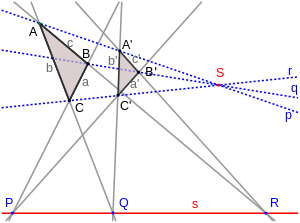
\includegraphics[scale=0.5]{desargues.png}  
\end{center}

\lstset{language=Python}

\begin{lstlisting}
 def desarguasian_plane(P):
    F=0
    T=0
    blocks = P._blocks
    k = len(blocks[0])-1
    inter_matrix = matrix(ZZ,k**2 + k + 1)
    line_matrix = matrix(ZZ, k**2 + k + 1)
    for n,b in enumerate(blocks):
        for i in b:
            for j in b:
                line_matrix[i,j] = n
        for m,c in enumerate(blocks):
            inter_matrix[m,n] = set(b).intersection(c).pop()
    from itertools import product
    for a1,b1,c1 in product(range(k**2 + k + 1), repeat = 3):
        if a1==b1 or b1==c1:
            continue
        if inter_matrix[a1,c1]==inter_matrix[a1,b1]:
            continue
        for a2,b2,c2 in product(range(k**2 + k + 1), repeat = 3):
            if a2==b2 or b2==c2:
                continue
            if inter_matrix[a2,c2]==inter_matrix[a2,b2]:
                continue
            A = line_matrix[a1,a2]
            B = line_matrix[b1,b2]
            C = line_matrix[c1,c2]
            concurrent = inter_matrix[A,B] == inter_matrix[B,C]
            BC1 = line_matrix[b1,c1]
            BC2 = line_matrix[b2,c2]
            p = inter_matrix[BC1,BC2]
            AC1 = line_matrix[a1,c1]
            AC2 = line_matrix[a2,c2]
            q = inter_matrix[AC1,AC2]
            AB1 = line_matrix[b1,a1]
            AB2 = line_matrix[b2,a2]
            r = inter_matrix[AB1,AB2]
            aligned = line_matrix[p,q] == line_matrix[q,r]
            if aligned != concurrent:
                print (a1,b1,c1)
                print (a2,b2,c2)
                print (p,q,r)
                print (A,B,C)
                print 'aligned {}, concurrent{}'.format(aligned,concurrent)
\end{lstlisting}
\end{document}
